\subsection{\textbf{Quick Elimination Convex Hull:}}

Quick Elimination optimizes Graham Scan by dividing the point set into smaller subsets. This approach reduces the time complexity for specific cases.

\begin{figure}[h]
    \centering
    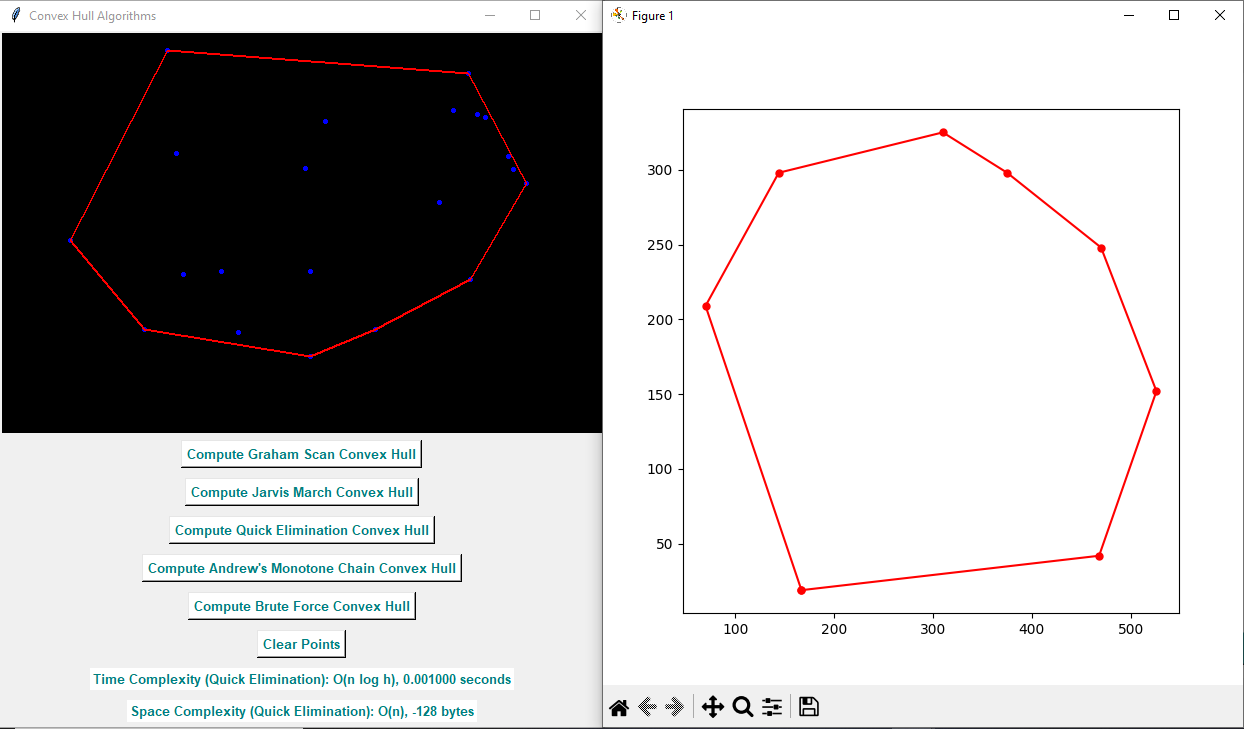
\includegraphics[width=1\linewidth]{quick elimination.PNG}
    \caption{Quick Elimination}
    \label{fig:quick elimination}
\end{figure}

\vspace{10pt}

\subsection{\textbf{Andrew’s Monotone Chain Convex Hull:}}

Andrew’s Algorithm offers a balance between efficiency and simplicity. It performs well for moderate-sized datasets.

\begin{figure}[h]
    \centering
    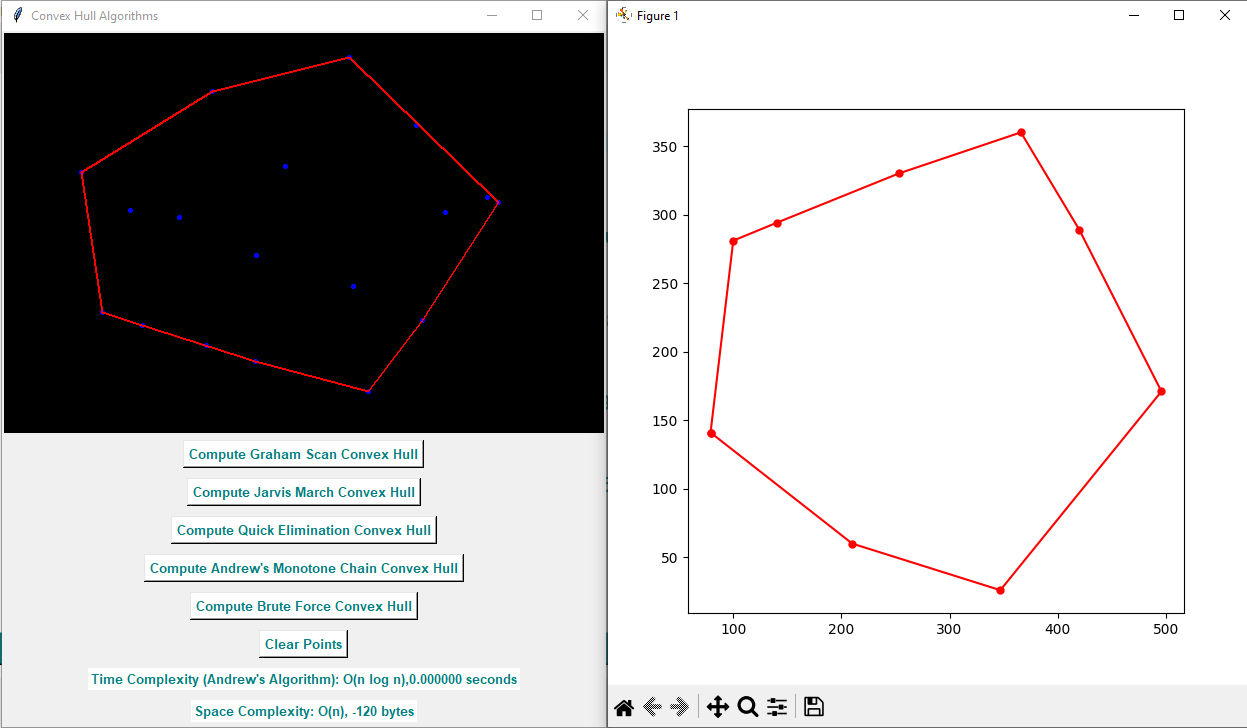
\includegraphics[width=1\linewidth]{andrew.PNG}
    \caption{Andrew's Monotone Chain}
    \label{fig:andrew}
\end{figure}

